\documentclass[12pt]{article}

\usepackage{parskip}
\usepackage{mdframed}
\usepackage{hyperref}
\usepackage{graphicx}
\usepackage{subcaption}
\usepackage{subfiles}
\usepackage{import}
\usepackage{mdframed}
\usepackage{amsmath}
\usepackage{multicol}
\usepackage{amsfonts}
\usepackage{tikz}
\usepackage{tcolorbox}
\usepackage{multirow}

\title{Formula Sheet}
\author{Nikesh Kumar}
\date{6th February,2020}

\newtcolorbox{notes}{
  title=NOTE,
  colframe=black,
  colback=white,
  arc=6pt,
  fonttitle=\rmfamily
}

\begin{document}
\maketitle
\thispagestyle{empty}
\newpage
\tableofcontents
\thispagestyle{empty}
\newpage
\pagenumbering{arabic}
\section{Partial Derivatives}
\subsection{Euler's Theorem}
Assuming $z$ to be \underline{homogenous} i.e. \fbox{$z=x^nf(y/x)$} ,
\[ x\frac{\partial z}{\partial x} + y\frac{\partial z}{\partial y} = nu \]
On \underline{partially differentiating}\footnote{Important proof} above equation wrt $x$ and $y$ we get,
\[ x^2\frac{\partial^2 z}{\partial x^2} + y^2\frac{\partial^2 z}{\partial y^2} + 2xy\frac{\partial^2 z}{\partial x\partial y} = n(n-1)z \]

\subsection{Total Differentiation}
\vspace{0.5cm}
\begin{itemize}
\item 
{\renewcommand{\arraystretch}{1.5}
\begin{tabular}{|c|c|c|}
\hline
$z=f(x,y)$&$x=\phi(t)$&$y=\phi(t)$ \\
\hline
\end{tabular}}
\begin{center}
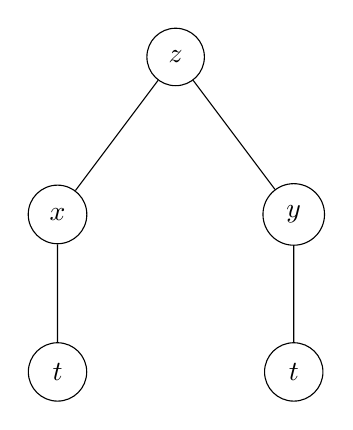
\begin{tikzpicture}[every node/.style={circle,inner sep=0.5em,draw=black}]
    \node (A) at (1.5,2) {$z$};
    \node (B) at (0,0) {$x$};
    \node (C) at (3,0) {$y$};
    \node (D) at (0,-2) {$t$};
    \node (E) at (3,-2) {$t$};

    \draw
        (A) -- (B)
        (A) -- (C)
        (B) -- (D)
        (C) -- (E);
\end{tikzpicture}
\end{center}
\[\text{\textbf{Differentiation: }} \frac{dz}{dt}=\frac{dz}{dx}\frac{dx}{dt}+\frac{dz}{dy}\frac{dy}{dt}\]    
\newpage
\item 
{\renewcommand{\arraystretch}{1.5}
\begin{tabular}{|c|c|c|}
\hline
$z=f(x,y)$&$x=\phi(u,v)$&$y=\phi(u,v)$ \\
\hline
\end{tabular}}
\begin{center}
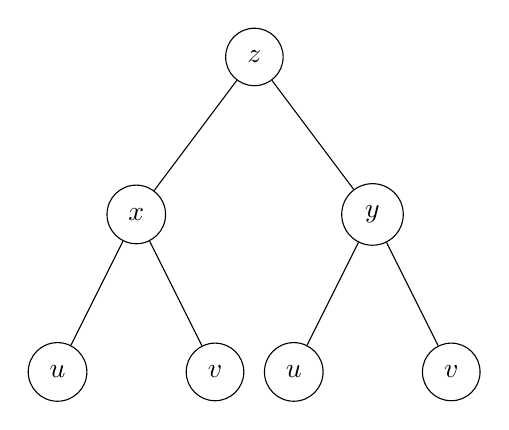
\begin{tikzpicture}[every node/.style={circle,inner sep=0.5em,draw=black}]
    \node (A) at (1.5,2) {$z$};
    \node (B) at (0,0) {$x$};
    \node (C) at (3,0) {$y$};
    \node (D1) at (-1,-2) {$u$};
    \node (D2) at (1,-2) {$v$};
    \node (E1) at (2,-2) {$u$};
    \node (E2) at (4,-2) {$v$};

    \draw
        (A) -- (B)
        (A) -- (C)
        (B) -- (D1)
        (B) -- (D2)
        (C) -- (E1)
        (C) -- (E2);
\end{tikzpicture}
\end{center}
\begin{align*}
\text{\textbf{Differentiation: }} &\frac{dz}{dt}=\frac{dz}{dx}\frac{dx}{du}+\frac{dz}{dy}\frac{dy}{du} \\
\text{\textbf{}} &\frac{dz}{dt}=\frac{dz}{dx}\frac{dx}{dv}+\frac{dz}{dy}\frac{dy}{dv} \\   
\end{align*}

\item Implicit Equation \fbox{$f(x,y) = c$}
\end{itemize}

\subsection{Mean Value Theorems}
\begin{itemize}
\item Rolle's Mean Value Theorem
\begin{itemize}
\item $f(x)$ is continuous in $[a,b]$
\item $f(x)$ is differentiable in $(a,b)$
\item $f(a)=f(b)$
\end{itemize}
There exists a $c\in(a,b)$ such that \fbox{$f'(c)=0$}

\item Lagrange's Mean Value Theorem
\begin{itemize}
\item $f(x)$ is continuous in $[a,b]$
\item $f(x)$ is differentiable in $(a,b)$
\end{itemize}
There exists a $c\in(a,b)$ such that \fbox{$f'(c)=\frac{f(b)-f(a)}{b-a}$}

\item Cauchy's Mean Value Theorem
\begin{itemize}
\item $f(x)\;\&\;g(x)$ is continuous in $[a,b]$
\item $f(x)\;\&\;g(x)$ is differentiable in $(a,b)$
\item $g'(x) \neq 0$
\end{itemize}
There exists a $c\in(a,b)$ such that \fbox{$\frac{f'(c)}{g'(c)}=\frac{f(b)-f(a)}{g(b)-g(a)}$}
\end{itemize}

\subsection{Taylor's Theorem}

\fbox{Single Variable}
\[f(x)=f(a)+(x-a)f'(a)+\frac{(x-a)^2}{2!}f''(a)\dots\]
$\diamondsuit$ \fbox{Mclaurin's Series}
\[f(x)=f(0)+xf'(0)+\frac{x^2}{2!}f''(0)\dots\]

\fbox{Two Variables}
\begin{align*}
f(x,y)=f(a,b)+\left[(x-a)\,f_x'(a,b)+(y-b)\,f_y'(a,b)\right]\\
+\frac{1}{2!}\left[(x-a)^2\,f_{xx}(a,b)+2(x-a)(y-b)\,f_{xy}(a,b)+(y-b)^2\,f_{yy}(a,b)\right]\\
+\frac{1}{3!}[(x-a)^3f_{xxx}\,f(a,b)+3(x-a)^2(y-b)\,f_{xxy}(a,b)\\
+3(x-a)(y-b)^2\,f_{xyy}(a,b)+(y-b)^3\,f_{yyy}(a,b)
\end{align*}
$\diamondsuit$ \fbox{Mclaurin's Series}
\begin{align*}
f(x,y)=f(0,0)+\left[x\,f_x'(0,0)+y\,f_y'(0,0)\right]\\
+\frac{1}{2!}\left[x^2\,f_{xx}(0,0)+2xy\,f_{xy}(0,0)+y^2\,f_{yy}(0,0)\right]\dots
\end{align*}

\begin{notes}
Try to memorise all the expansions of $sin\,x,cos\,x,log\,x,e^x,a^x$, will be helpful a lot in solving limits and indeterminate forms
\end{notes}

\begin{notes}
Leibinitz Rule(for $n^{th}$ differentiation)\footnote{$U_n$ denotes $n^{th}$ derivative of $U$}
\[(UV)_n= \binom{n}{0}UV_n+\binom{n}{1}U_1V_{n-1}+\binom{n}{2}U_2V_{n-2}\dots+\binom{n}{n}U_nV\]
\end{notes}

\subsection{Maxima \& Minima}
\begin{itemize}
\item $f_x=0$\\
      $f_y=0$
\item $r=f_{xx}$\\
      $s=f_{xy}$\\
      $t=f_{yy}$

$$ rs- t^2 = \left\{
    \begin{tabular}{cp{4cm}c}
        \multirow{2}{*}{$>0$} && $\text{Minima }(r>0)$ \\
        && $\text{Maxima }(r<0)$ \\
        $<0$ && \text{Saddle Point} \\
        $=0$ && \text{No conclusion}
    \end{tabular}
\right.
$$
\end{itemize}

\subsection{Lagrange's Method of Undetermined Multipier}
Let $f(x,y,z)$\footnote{Here $f$ is the function to be minimised} be subject to the condition $\phi(x,y,z)=0$ then using concept of linear combinations,
\begin{center}
\fbox{$F = f(x,y,z) + \lambda\,\phi(x,y,z)$}
\end{center}
where $\lambda\;\in\;\mathbb{R}$. To get the minimum solve the following equations,
$$\frac{\partial F}{\partial x}=0\quad\frac{\partial F}{\partial y}=0\quad\frac{\partial F}{\partial z}=0$$

\subsection{Errors and Approximations}
Here $\delta f$ denotes the error in $f$.
$$\delta f=\frac{\partial f}{\partial x}\delta x+\frac{\partial f}{\partial }\delta y$$

\begin{notes}
A better way would be taking log and then differentiating as shown below.
\vspace{0.3cm}
\begin{tcolorbox}
\[V = \frac{4}{3}\pi r^3\]
[Taking $\log$] \\
$\Rightarrow log\,V = log(\frac{4}{3})+\log\,\pi+3\log\,r$
\vspace{0.3cm}

[Taking derivative] \\
$\Rightarrow \frac{1}{V}\partial V = 3\frac{1}{r}\partial r$ 
\vspace{0.15cm}

$\Rightarrow \frac{\partial V}{V} = 3\frac{\partial r}{r}$
\vspace{0.3cm}

[Considering $\partial x \sim  \delta x$] \\
$\Rightarrow \frac{\delta V}{V} = 3\frac{\delta r}{r}$
\end{tcolorbox}
\end{notes}
\newpage

\section{3D Geometry}
\subsection{Sphere}
\begin{itemize}
\item Basic Equation: \fbox{$x^2+y^2+z^2+2fx+2gy+2hz+d=0$}
\item Center: \fbox{$(-f,-g,-h)$} \vspace{0.1cm} \\
      Radius: \fbox{$\sqrt{f^2+g^2+h^2-d}$}
\item Other forms of equations:
\begin{itemize}
    \item When $x_o,y_o,z_o$ is the centre and r is radius. \\
    \fbox{$(x-x_o)^2+(y-y_o)^2+(z-z_o)^2=r^2$}

    \item When $x_1,y_1,z_1$ \& $x_2,y_2,z_2$ are diametrically opposite ends. \\
    \fbox{$(x-x_1)(x-x_2)+(y-y_1)(y-y_2)+(z-z_1)(z-z_2)=0$}    
\end{itemize}
\item Intersection of Plane($T=0$) with Sphere($C=0$) the the equation of family of spheres is given by \fbox{$S+\lambda T = 0$}
\begin{itemize}
    \item Center: \fbox{$(x,y,z)$}\quad
          Radius: \fbox{$r^2-p^2$}
    \begin{notes}
    Direct formula for $p$ where $x_o,y_o,z_o$ is the centre of the circle and $ax+by+cz+d=0$ is equation of the plane:
    $$p = \left|\frac{ax_o+by_o+cz_o+d}{\sqrt{a^2+b^2+c^2}}\right| $$

    Equation of line passing from center normal to the plane
    $$\frac{x-x_p}{a}=\frac{y-y_o}{b}=\frac{z-z_o}{c}$$
    
    For $k=1$, on solving we get point on plane \& $k=2$, we get mirrored point in plane
    $$\frac{x-x_p}{a}=\frac{y-y_o}{b}=\frac{z-z_o}{c} = \frac{-(ax_o+by_o+cz_o+d)}{a^2+b^2+c^2}\times k$$
    \end{notes}
\end{itemize}
\item Orthogonal Spheres

Let $d$ be the distance between the centres and $r_1$ and $r_2$ be the radii of the two spheres. Then condition for orthogonal circles would be:
\begin{center}
\fbox{$d^2 = r_1^2 + r_2^2$}
$\Rightarrow 2f_1f_2+2g_1g_2+2h_1h_2=d_1+d_2$
\end{center}

\item Tangent to Sphere

If the tangent touches the circle $x^2+y^2+z^2+2fx+2gy+2hz+d=0$ at point $(x_1,y_1,z_1)$ then the equation of the tangent would be:

\begin{center}
\fbox{$xx_1+yy_1+zz_1+f(x+x_1)+g(y+y_1)+h(z+z_1)=0$}
\end{center}
\end{itemize}
\end{document}